
\documentclass[english]{article}
%\documentclass[aps,pra,twocolumn,english]{revtex4}
%\documentclass[english]{iopart}
\usepackage[T1]{fontenc}
\usepackage[latin9]{inputenc}
\usepackage{babel}
\usepackage{graphicx,amsmath,amssymb,color}
\usepackage[normalem]{ulem}
\usepackage{amsfonts}
\usepackage[toc,page]{appendix}
%\usepackage[ocgcolorlinks,colorlinks=true,linkcolor=blue,citecolor=red]{hyperref}
\usepackage{hyperref}
\usepackage{latexsym}
\usepackage{amsfonts}
\usepackage{algpseudocode}
\usepackage{amsthm}
\usepackage{mathrsfs}
\usepackage{natbib}
\usepackage{color,verbatim}
\usepackage{psfrag}
\bibliographystyle{unsrt}
%\bibliographystyle{acm}
%\bibliographystyle{unsrtnat}
%\usepackage[style=numeric]{biblatex}

\usepackage{subcaption} % allows for subfigures


\usepackage[svgnames]{xcolor}
\usepackage{tikz}

\usepackage{algorithm}


%\input{tikzit/tikz_preamble.tex}  % load separately defined tikz preamble


\newcommand{\bra}[1]{\langle#1 |}
\newcommand{\ket}[1]{|#1 \rangle}
\newcommand{\braket}[2]{\left \langle #1 \mid #2 \right \rangle}
\newcommand{\bigbraket}[2]{\left \langle #1 \middle\vert #2 \right \rangle}
\newcommand{\ketbra}[2]{\vert #1 \rangle \! \langle #2 \vert}
\newcommand{\overlap}[2]{\left \langle #1 | #2 \right\rangle}
\newcommand{\average}[1]{\langle #1 \rangle}
\newcommand{\sandwich}[3]{\left \langle #1 \mid #2 \mid #3 \right\rangle}
\newcommand{\innerprod}[2]{\left \langle #1 | #2 \right\rangle}

\begin{document}


\title{Non-linear optics}
\author{Nicholas Chancellor}


\maketitle


\today % added for drafting, remove in final version


{\small Disclaimer: lecture notes may contain ``typo'' type errors (factors of $2$, minus signs, etc...) if something like this looks wrong there is a good chance it is, please let me know}

These notes are based on Gerry and Knight as well as ``Nonlinear Optics'' by Robert Boyd ISBN: 978-0-12-369470-6, available for purchase at\footnote{while this is a good book in general I don't necessarily think that everyone needs a copy of  it the way we all have a copy of G+K (get QCI to buy you one if you don't already have it), maybe only get it if you want to know how the experiments work}:\\ \href{https://www.elsevier.com/books/nonlinear-optics/boyd/978-0-12-369470-6}{https://www.elsevier.com/books/nonlinear-optics/boyd/978-0-12-369470-6}, quantum field theory sketch based on Anthony Zee, Quantum Field Theory in a Nutshell, available for purchase at\\ \href{https://press.princeton.edu/books/hardcover/9780691140346/quantum-field-theory-in-a-nutshell}{https://press.princeton.edu/books/hardcover/9780691140346/quantum-field-theory-in-a-nutshell} (we probably won't need this for QCI stuff, but could be worth getting for your own curiosity)

\section{Non-linear versus linear optics}
\begin{itemize}
\item Why are we learning this? Non-linear optics is the basis of many real optical components, while this lecture is mostly the theory behind non-linear optics, it will build a groundwork for understanding components such as optical parametric oscillators (OPOs), accusto- and electro- optical modulators (AOMs and EOMs), Raman amplifiers, and many others
\item Non-linear optics involves considering optical effects which involve the response of materials beyond the regime where the response can be approximated as linear (i.e.~something which obeys the superposition principle)
\item But quantum mechanics is a fundamentally linear theory\footnote{Ignoring whatever is going on with quantum gravity, no one really knows how that works}, where does this non-linearity come from?  Many (or even a few) linear systems acting together can be approximated as something non-linear, and it is often the only way to make them tractable
\item Any physical system responds in a non-linear way if you drive it hard enough, even the vacuum, as we will see later, also get non-linear behaviour near resonances
\item A nice non-quantum/non-optical example is a simple pendulum, at low amplitudes well approximated as a harmonic oscillator and frequency is independent of amplitude, at large amplitudes the frequency starts to depend on amplitude, (meaning the oscillations no longer obey a superposition principle)
\item In principle, ``driving hard enough'' can either mean a lot of photons (leading to a strong $E$ field), or can mean few photons at very high energy, the first case is the one which is interesting to us, I won't talk about the second one (neither does Boyd)
\item Even a few photons near an atomic resonance act in a non-linear way (one can be absorbed and then the others can't)
\item In general non-linear differential equations are very hard to solve, can't directly use the standard matrix methods we are used to from QM
\item Expand in terms of higher order interactions, get susceptibilities for each order of interactions, linear susceptability $\chi^{(1)}$ contributes terms of the form $\chi^{(1)}\hat{a}^\dagger\hat{a}$ second order susceptability contributes terms which look like $\chi^{(2)}\hat{a}_x^\dagger\hat{a}_y^\dagger\hat{a}_z$ (and the conjugate of these terms, subscripts added to emphasise that these cannot all be the same mode by conservation of energy), third order $\chi^{(3)}$ is the same with three terms
\item Because higher order terms involve more photons they correspond to higher dimensional tensors, $\chi^{(1)}$ is a vector, $\chi^{(2)}$ is a matrix $\chi^{(3)}$, a rank 3 tensor, etc... Usually only $1$, $2$ and $3$ are relevant $3$ because for many systems $\chi^{(2)}$ is identically zero by symmetry
\item Even though squeezing operators only involve $\hat{a}^{(\dagger)}\hat{a}^{(\dagger)}$, they either involve terms either both with or both without daggers, these violate conservation of energy so in practice are usually implemented using terms of the form $\hat{a}_p\hat{a}_1^{\dagger}\hat{a}_1^{\dagger}+\hat{a}^\dagger_p\hat{a}_1\hat{a}_1$, how this can be done can be found in  section 7.2 of G+K, see particularly equation 7.84
\item For squeezing operator generation it is usually convenient to use such a strong field (the pump) that photon loss of than field can be ignored and it can be treated as classical, leaving the familiar squeezing operation $\hat{a}_1^{\dagger}\hat{a}_1^{\dagger}+\hat{a}_1\hat{a}_1$
\end{itemize}

\section{First order (linear) susceptibility of an atomic system}
\begin{itemize}
\item This is actually deriving the linear response of an atom, but shows how the non-linear versions work (paraphrasing/condensing the full calculation from sections 3.4 and 3.5 of Boyd (full details there))
\item Susceptibility relates to the off-diagonal elements of the density matrix when driven by an electric field (treated as classical in this calculation)
\item Atomic system which allows a decay process (3.4.1 in Boyd) ``eq'' denotes equilibrium state (usually either ground state or thermal state, but always with zero off diagonal elements):
\begin{equation}
\frac{\partial \rho_{nm}}{\partial t}=\frac{i}{\hbar}\left[\hat{H},\hat{\rho}\right]-\gamma_{nm}\left(\rho_{nm}-\rho^{(eq)}_{nm}\right)
\end{equation}
\item Hamiltonian can be treated as two parts (combination of Eq.~3.4.2 in Boyd)
\begin{equation}
\hat{H}=\hat{H}_0+\hat{V}
\end{equation}
\item $\hat{H}_0$ is diagonal causes an oscillation at frequency $\omega_{nm}$ and $\hat{V}=\hat{\mu}E(t)$, the field times the susceptibility 
\item Assume system is in $\hat{\rho}=\hat{\rho}^{(eq)}$ except for effect of the field, and apply first order perturbation theory ($\hat \rho^{(1)}$ represents the difference from the equilibrium, so not a proper density matrix):
\begin{equation}
\frac{\partial}{\partial t}\rho_{nm}^{(1)}=(i\omega_{nm}+\gamma_{nm})\rho^{(1)}-i\hbar [\hat{V},\hat{\rho}^{(0)}]_{nm}
\end{equation}
\item First term gives an exponential envelope of $\exp\left[(i \omega_{nm}+\gamma_{nm})t \right]$, so equation is easier to solve by assuming the form $\rho_{nm}^{(1)}=S_{nm}^{(1)}\exp\left[(i \omega_{nm}+\gamma_{nm})t \right]$
\item Some algebra gives (3.5.1 in Boyd)
\begin{align}
\rho^{(1)}_{nm}(t)=\nonumber \\
\exp\left[-(i\omega_{nm}+\gamma_{nm})t \right]\int_{-\infty}^tdt'\frac{-i}{\hbar}\left[\hat{V}(t'),\hat{\rho}^{(eq)}\right]_{nm}\exp\left[(i \omega_{nm}+\gamma_{nm}\right)t']
\end{align}
\item In the case of an electromagnetic wave at frequency $\omega_p$, \\$\hat{V}_{nm}(t)=\mu_{nm}E(\omega_p)\exp\left[i\omega_p t \right]$
\item Having plugged this in, the equation becomes (3.5.7 in Boyd)
\begin{align}
\rho^{(1)}_{nm}(t)=\frac{i}{\hbar}(\rho^{(eq)}_{mm}-\rho^{(eq)}_{nn})\mu_{nm}\sum_p E(\omega_p) \nonumber \\ \times\exp\left[-(i\omega_{nm}+\gamma_{nm})t \right]\int_{-\infty}^tdt'\exp\left[(i (\omega_{nm}-\omega_p)+\gamma_{nm}\right)t']
\end{align}
\item Boyd just quotes a result to evaluate the integral, but the trick to solve it is interesting (and I happen to know it), the integral can be rephrased
\begin{align}
\int_{-\infty}^tdt'\exp\left[(i (\omega_{nm}-\omega_p)+\gamma_{nm}\right)t']=\nonumber \\
\int_{-\infty}^{\infty}dt'\exp\left[-\omega_p t'\right]\exp\left[(i \omega_{nm}+\gamma_{nm}\right)t']\Theta(t-t')= \\
\mathcal{F}\left[ \exp\left[(i \omega_{nm}+\gamma_{nm}\right)t']\Theta(t-t') \right]
\end{align}
\item Where $\mathcal{F}$ indicates a Fourier transform and $\Theta$ is the Heviside function $\Theta(x>0)=1$, $\Theta(x<0)=0$, the trick is then to realize that the Heviside theta is the antiderivative of the Dirac delta (the Forier transform of which is constant), and in the Fourier domain, antidiferentiation can be represented by dividing by $\omega$ so $\mathcal{F}\left[ \Theta(t)\right]=\frac{1}{\omega}$,  this can then be combined with the fact that multiplication in the real domain is convolution in the Fourier domain, so multiplying by the exponential just shifts the position of the function in the complex plane
\item The final result for the density matrix element is (3.5.9 in Boyd)
\begin{equation}
\rho_{nm}^{(1)}=\frac{(\rho^{(eq)}_{mm}-\rho^{(eq)}_{nn})}{\hbar}\sum_p\frac{\mu_{nm}E(\omega_p)e^{i\omega_p t}}{(\omega_{nm}-\omega_p)-i\gamma_{nm}}
\end{equation}
\item From here the linear susceptability at a frequency $\omega_p$ can be derived by dividing out the electric field, multiplying by another factor of the dipole moment (since the effect of the density matrix element on the field will depend on this along with some physical constants to get the units right), and multplying by the number density $N$ of atoms the light encounters, the result is (3.5.13 in Boyd) 
\begin{equation}
\chi^{(1)}(\omega_p)=\frac{N}{\epsilon_0\hbar}\sum_{nm}(\rho^{(eq)}_{mm}-\rho^{(eq)}_{nn})\frac{\mu_{mn}\mu_{nm}}{(\omega_{nm}-\omega_p)-i \gamma_{nm}} \label{eq:full_first_order_suscept}
\end{equation}
\item Assuming we start in level $a$ and only one term coming from level $n$ contributes (and doing some minor algebra), we have (3.5.21in Boyd)
\begin{equation}
\chi^{(1)}(\omega_p)=\frac{N}{\epsilon_0\hbar}\mu_{an}\mu_{na}\frac{(\omega_{na}-\omega_p)+i \gamma_{na}}{(\omega_{na}-\omega_p)^2+\gamma^2_{nm}} \label{eq:suscept_2lvl}
\end{equation}
\item What does this mean physically, a few observations 
\begin{itemize}
\item The effect tends to be stronger closer to resonance, but a transition with frequency $\omega_{nm}$ does contribute at any frequency $\omega_p$
\item The imaginary part (corresponding to absorption) has a width which depends on the strength of the decay, transitions with stronger decay can absorb photons further off resonance
\item We actually made very few assumptions about the nature of the system, will be broadly applicable (even to the vacuum)
\item No reason we can't consider processes involving more photons in a similar way (this is where non-linear optics comes in)
\end{itemize}
\end{itemize}

\section{(non)parametric processes and virtual energy levels}

\begin{itemize}
\item One way to physically interpret the previous section: there is a short lived ``virtual'' energy level $\omega_p$ away from our starting level which becomes populated for a short period of time (violates energy conservation, but this is ok thanks to time-energy uncertainty)
\item The (real part of the) linear susceptibility from Eq.~ \ref{eq:suscept_2lvl} can be understood as a photon being briefly absorbed into a virtual energy level and re-emitted as shown in the diagram below (solid lines are real energy levels, virtual ones shown as dashed lines

\begin{centering}
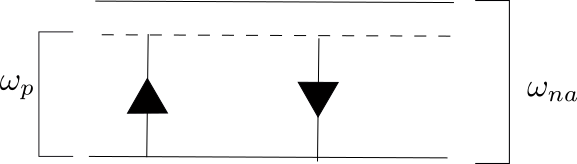
\includegraphics[width=0.5 \columnwidth]{cartoons/one_component_linear_suscept.png}
\par
\end{centering}
\item We now have a diagrammatic way to understand these processes, what if we consider a more complicated processes involving more photons and levels, for example parametric down conversion, where one photon is absorbed and two are emitted (half the frequency for simplicity in this case) in our familiar QO language $\hat{a}_1\hat{a}^\dagger_2\hat{a}^\dagger_2$

\begin{centering}
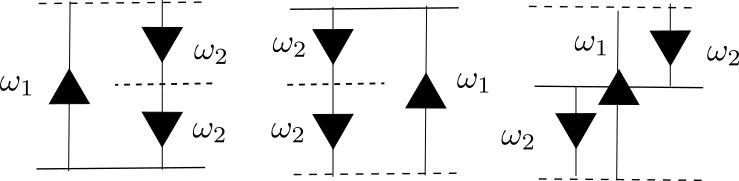
\includegraphics[width=0.5 \columnwidth]{cartoons/parametric_down_conversion_levels.png}
\par
\end{centering}
\item All three processes must be considered to get an accurate value of the second order susceptability which controls this process $\chi^{(2)}(\omega_1,\omega_2)$, otherwise calculations proceed similar to Eq.~\ref{eq:full_first_order_suscept} but with one of these terms for each virtual level involved (I am not going to do this in detail but Boyd does)
\item Can also involve processes which start and end in different (real) energy levels (n.b. virtual energy levels can only exist for a short time, we cannot end in them)
\begin{itemize}
\item Interactions which leave the matter the photons interact with in the same starting state are called \textbf{parametric}, these processes must conserve the total energy of the photons since the matter does not absorb or emit energy
\item Interactions where the matter ends in a different state are \textbf{non-parametric}, the energy of the photons is generally not conserved
\end{itemize}
\item Momentum conservation has important consequences for which processes actually happen, as we will see later when discussing phase matching 
\item The simplest non-parametric process is emitting or absorbing a photon, the next simplest is probably Raman scattering, which follows a diagram like linear susceptability, but the matter ends in a different state, leading to a photon with lower (left) or higher (right) energy\footnote{For an accurate calculation one would have to consider all permutations of this, including those where the virtual level is lower in energy}
\begin{centering}
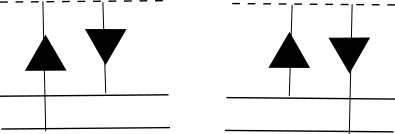
\includegraphics[width=0.5 \columnwidth]{cartoons/Raman_levels.png}
\par
\end{centering}
\item For an interesting example (thanks to my colleagues at Durham) of non-parametric processes can be used in imaging terahertz radiation (a range of frequencies were normal imaging methods don't work well), see\\ \href{https://journals.aps.org/prx/abstract/10.1103/PhysRevX.10.011027}{https://journals.aps.org/prx/abstract/10.1103/PhysRevX.10.011027}
\item The underlying derivation relies on perturbation theory,which can be applied in many contexts, here is an example where it can be applied in a transverse Ising model \href{https://arxiv.org/abs/1812.07885}{https://arxiv.org/abs/1812.07885}
\end{itemize}

\section{Applying the same concept to the quantum vacuum}
\begin{itemize}
\item The derivation here doesn't make any assumptions on what kind of material the photons are interacting with, what happens if we consider photons interacting with the vacuum
\begin{itemize}
\item The vacuum has resonances/energy levels (particles pairs can be created)
\item Photons couple to these energy levels (a cosmic ray can decay into massive particles)
\item Just like we did with virtual energy levels we should have a systematic way of characterising the interactions (this is actually what Feynmann diagrams are)
\end{itemize}
\item Sketch of how to do this\footnote{For the details of how all the pieces of this calculation would actually work, see Zee, particularly I.7, II.1, II.2}: photon-photon scattering process, photons don't interact directly, but they can create (virtual) electron-positron pairs\footnote{These will have the leading order contribution since the electron (and its anti-particle) are the least massive particles which couple to photons} which interact, four in total, two incoming, two outgoing
\item This process can be represented in terms of virtual energy levels (left) or Feynmann diagram (right)

\begin{centering}
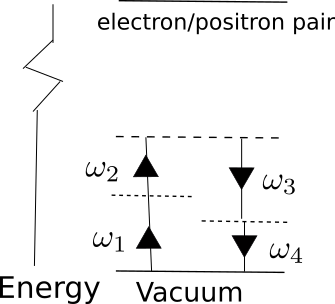
\includegraphics[width=0.45 \columnwidth]{cartoons/photon-photon_virt_level.png}
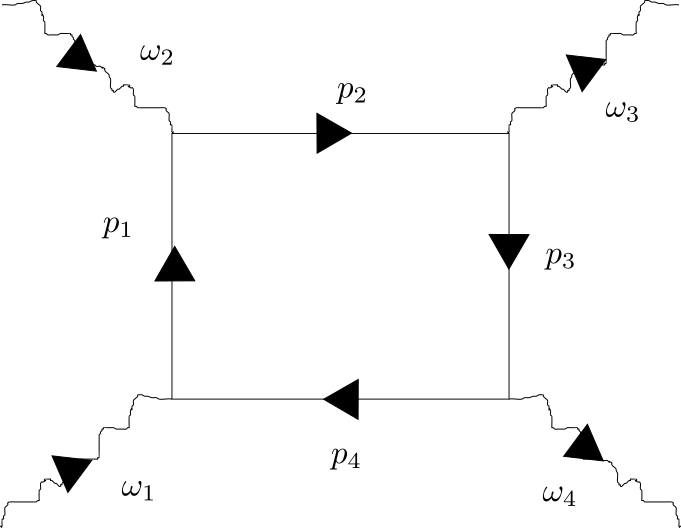
\includegraphics[width=0.45 \columnwidth]{cartoons/photon-photon.png}
\par
\end{centering}
\item By energy/momentum conservation, $\omega_4$ and the direction of this photon are set by the other three, therefore we have three constraints on the four momentum terms $p_{1-4}$, we have a degree of freedom to integrate over
\item This leads to an integral which looks like (details can be found in Zee): 
\begin{align}
\int d^4p_1 (...)\frac{1}{\not{p}_1-m_e+i\epsilon}\frac{1}{\not{p}_2-m_e+i\epsilon}\frac{1}{\not{p}_3-m_e+i\epsilon}\frac{1}{\not{p}_4-m_e+i\epsilon}
\end{align}
\item Here $(...)$ indicates constraints on some of the momentum variables based on the values of the others and photon momentum, as well as some physical constants and summation over permutations of the input photons, the slash $\not{p}$ notation relates to some matrix tricks which are needed to represent spin $\frac{1}{2}$ particles (details can be found in Zee), $\epsilon$ is the decay rate of the electron/positron, which will go to zero since they are stable particles, but is needed for technical reasons related to contour integration
\item Easiest to understand by realising that in the 4d relativistic setting the four-momentum expectation $\average{\not{p}}$ is more like what we think of as total mass, a ``real'' electron must obey the Dirac equation $(\not{p}-m)\ket{\psi}=0$, but a virtual particle does not need to (called ``off shell'' in particle physics) as long as it only exists for a short period of time, however value decreases the further ``off shell'' we become, since visible light has much less energy than the electron mass, the cross section for visible photons is almost (but not exactly)  zero, and can be ignored in all real experiments that I know of
\item The derivation of the math of Feynmann diagrams actually starts from perturbation theory, just like we did here!
\item Field theory can be and is often applied in condensed matter systems as well (Zee is focused on high energy physics so can be misleading here)
\end{itemize}
\section{Back to the practical aspects: (quasi-) phase matching}
\begin{itemize}
\item While virtual energy levels don't have to obey energy or momentum conservation since they are short-lived, the incoming and outgoing photons do (or the photons+the matter in a non-parametric process), this puts a lot of constraints on what processes will or won't happen
\item Beneficial because it means that photons produced by non-linear processes will be produced in a set direction
\item For second order non-linearity using the convention of G+K ($\hat{a}_p\hat{a}^\dagger_s\hat{a}^\dagger_i+h.c.$) with $p$ (pump), $s$ (signal), and $i$ (idler) modes we have for parametric down conversion (equations 9.3 and 9.4 in G+K)
\begin{itemize}
\item Energy conservation $\hbar \omega_p=\hbar \omega_s+\hbar \omega_i$
\item Momentum conservation, aka phase matching $\hbar \vec{k}_p\approx \hbar \vec{k}_s+\hbar \vec{k}_i$ (approximate because of uncertainty due to finite length of medium)
\end{itemize}
\item  $\vec{k}_i$ are the wavenumbers (proportional to inverse wavelength, $|\vec{k}_i|=\frac{n(\omega_i)\omega_i}{c}$) of each wave, note that $n(\omega)$ is usually an increasing function with $\omega$  (normal dispersion) In chapter 2 Boyd devotes a lot of space to discussing the efficiency of non-liner processes when the second condition is only approximately met
\item Normal dispersion and phase matching imply that (without a special trick mentioned later) for parametric down conversion $\hat{a}_p\hat{a}_s^\dagger\hat{a}_i^\dagger$ there will be an angle between the signal and idler (see figure 9.2)
\item If we want entanglement, special directions need to be chosen so photons' polarisation cannot be inferred from direction (figures 9.3 and 9.4 in G+K)
\item To avoid this, we can use tricks such as birefringent media where wavenumber depends on polarisation allows us to make collinear beams (much easier for design of the rest of system) which obey the condition  $\frac{n_s\omega_s}{c}+\frac{n_i\omega_i}{c}=\frac{n_p\omega_p}{c}$ (eq. 2.3.3 in Boyd but with G+K naming convention), where $n$ is the refractive index each experiences based on its polarisation and frequency
\item Sometimes exact phase matching is just not possible, in this case quasi-phase matching must be employed, this can be done by slicing the medium and inverting the direction of some parts of the crystal with a specially chosen periodicity $\Lambda$, chapter 2.4 in Boyd
\item We probably don't need all the details of how this works (again Boyd goes into great detail) so much as to know that it is a very important part of the design of optical components, the math is basically just solving boundary condition equations and some differential equations, honestly it all has the feeling of being much easier to solve numerically 
\end{itemize}








\end{document}